% date: 2024-09-21
% Author: Bai Junhao
% Email: bjh2001@connect.hku.hk
% The University of Hong Kong

\section{I owe you a Yo-Yo}

\subsection{Question}
Repeat question 1 but this time with the sentence changed to “I owe you a Yo-Yo”.

\subsection{Answer}
Similarly, following the approach of Question 1, we get the spectrogram of the sentence “I owe you a Yo-Yo” as shown in Figure \ref{fig:Question2}.

\begin{figure}[H]
    \centering
    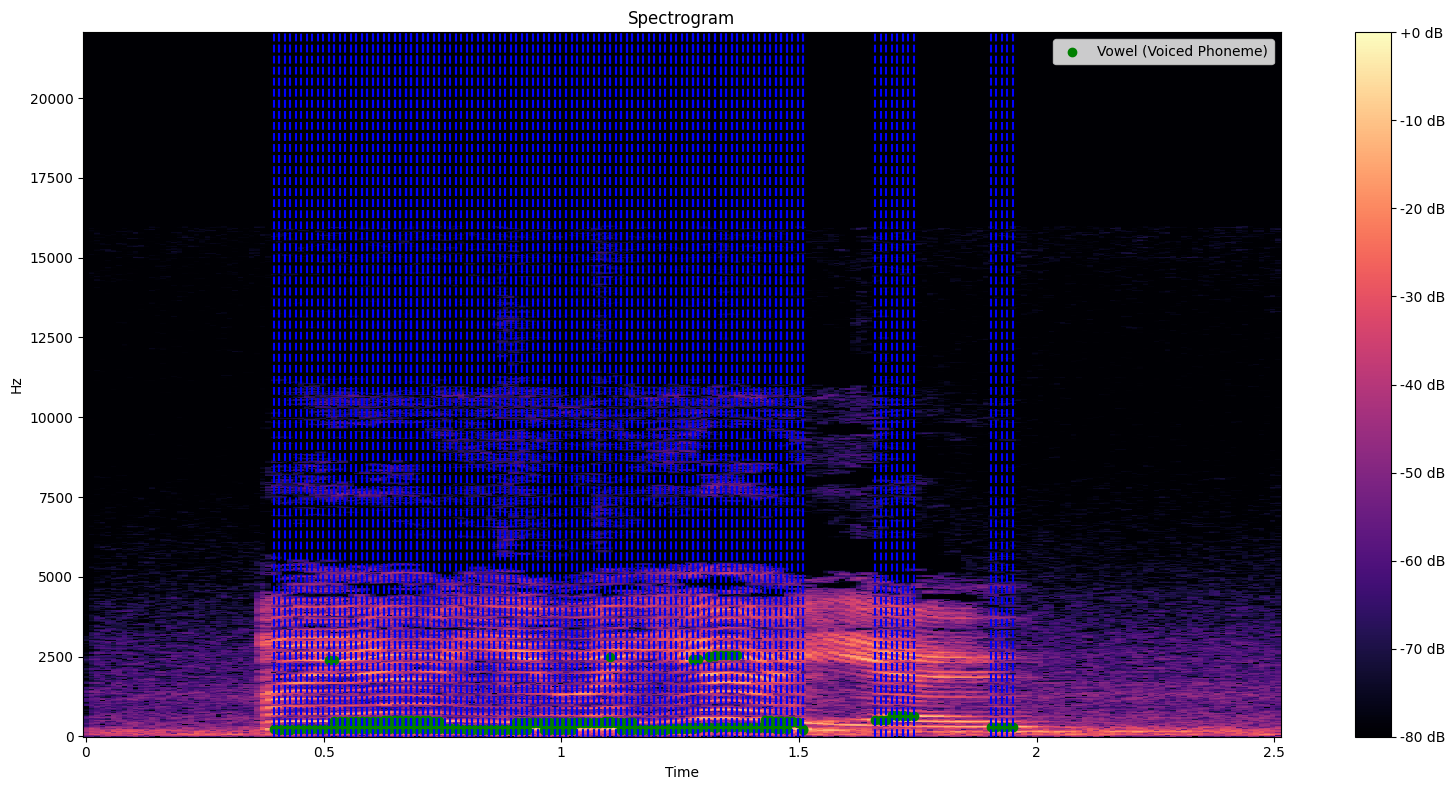
\includegraphics[width=\textwidth]{./img/Q2-1.png}
    \caption{Spectrogram of the sentence “I owe you a Yo-Yo”}
    \label{fig:Question2}
\end{figure}

As observed in the spectrogram, the vowels in this sentence exhibit a higher concentration, which complicates the task of identifying the boundaries of the syllables. This overlapping of vowel sounds can create ambiguity, making it challenging for listeners to pinpoint where one syllable ends and another begins. However, a careful examination reveals that certain vowel sounds are notably continuous throughout the sentence. For instance, the vowel in "I" from the phrase "I owe," the "o" in "owe," the "you" in "you a," and the "a" in "a Yo-Yo" all demonstrate a sustained presence.

In the spectrogram, these continuous vowel sounds are visually represented as straight lines, indicating their uninterrupted nature. This graphical representation suggests that these vowel sounds are held longer, contributing to the overall fluidity of the speech.

The number of vowels and consonants in this sentence are as follows:

\begin{table}[H]
    \centering
    \begin{tabular}{|c|c|c|}
        \hline
        \textbf{Voiced Phonemes} & \textbf{Phonetic Representation} & \textbf{Count} \\ \hline
        I  & I & /aɪ/ (1) \\ \hline
        owe & o, e & /əʊ/, /ʊ/ (2) \\ \hline
        you & u & /ju:/ (1) \\ \hline
        a & a & /eɪ/ (1) \\ \hline
        Yo-Yo & o, o & /əʊ/, /əʊ/ (2) \\ \hline
        \textcolor{red}{\textbf{Total}} & & \textcolor{red}{7} \\ \hline
    \end{tabular}
    \caption{Phonemes in "I owe you a Yo-Yo"}
\end{table}

There's no stop consonants in this sentence, as all the consonants are fricatives or approximants.

\newpage